\documentclass{beamer}
\mode<presentation>{
  \usetheme{Boadilla}
  \usefonttheme[onlylarge]{structurebold}
  \usefonttheme[stillsansseriflarge]{serif}
  \setbeamerfont*{frametitle}{size=\normalsize,series=\bfseries}
  % \setbeamertemplate{navigation symbols}{}
  \setbeamercovered{transparent}
}
\usepackage[english]{babel}
\usepackage[latin1]{inputenc}
\usepackage{times}
\usepackage[T1]{fontenc}
\usepackage{amsmath}
\usepackage{amssymb}
\usepackage{esint}
\usepackage{hyperref}
\usepackage{tikz}
\usepackage{xkeyval}
\usepackage{xargs}
\usepackage{xcolor}
\usepackage{verbatim}
\usepackage{listings}
\usepackage{multimedia}
\usepackage{bm}
\usepackage{siunitx}
\usetikzlibrary{
  arrows,
  calc,
  decorations.pathmorphing,
  decorations.pathreplacing,
  decorations.markings,
  fadings,
  positioning,
  shapes,
  arrows.meta
}
\usepgfmodule{oo}

\pgfdeclareradialshading{glow2}{\pgfpoint{0cm}{0cm}}{
  color(0mm)=(white);
  color(2mm)=(white);
  color(8mm)=(black);
  color(10mm)=(black)
}
\pgfdeclareradialshading{glow}{\pgfpoint{0cm}{0cm}}{
  color(0mm)=(white);
  color(5mm)=(white);
  color(9mm)=(black);
  color(10mm)=(black)
}

\begin{tikzfadingfrompicture}[name=glow fading]
  \shade [shading=glow] (0,0) circle (1);
\end{tikzfadingfrompicture}

\begin{tikzfadingfrompicture}[name=glow2 fading]
  \shade [shading=glow2] (0,0) circle (1);
\end{tikzfadingfrompicture}

\mode<handout>{
  \usepackage{pgfpages}
  \pgfpagesuselayout{4 on 1}[a4paper,landscape,border shrink=5mm]
  \setbeamercolor{background canvas}{bg=black!10}
}

\newcommand\pgfmathsinandcos[3]{%
  \pgfmathsetmacro#1{sin(#3)}%
  \pgfmathsetmacro#2{cos(#3)}%
}
\newcommand\LongitudePlane[3][current plane]{%
  \pgfmathsinandcos\sinEl\cosEl{#2} % elevation
  \pgfmathsinandcos\sint\cost{#3} % azimuth
  \tikzset{#1/.estyle={cm={\cost,\sint*\sinEl,0,\cosEl,(0,0)}}}
}
\newcommand\LatitudePlane[3][current plane]{%
  \pgfmathsinandcos\sinEl\cosEl{#2} % elevation
  \pgfmathsinandcos\sint\cost{#3} % latitude
  \pgfmathsetmacro\yshift{\cosEl*\sint}
  \tikzset{#1/.estyle={cm={\cost,0,0,\cost*\sinEl,(0,\yshift)}}} %
}
\newcommand\DrawLongitudeCircle[2][1]{
  \LongitudePlane{\angEl}{#2}
  \tikzset{current plane/.prefix style={scale=#1}}
  % angle of "visibility"
  \pgfmathsetmacro\angVis{atan(sin(#2)*cos(\angEl)/sin(\angEl))} %
  \draw[current plane] (\angVis:1) arc (\angVis:\angVis+180:1);
  \draw[current plane,dashed] (\angVis-180:1) arc (\angVis-180:\angVis:1);
}
\newcommand\DrawLatitudeCircleArrow[2][1]{
  \LatitudePlane{\angEl}{#2}
  \tikzset{current plane/.prefix style={scale=#1}}
  \pgfmathsetmacro\sinVis{sin(#2)/cos(#2)*sin(\angEl)/cos(\angEl)}
  % angle of "visibility"
  \pgfmathsetmacro\angVis{asin(min(1,max(\sinVis,-1)))}
  \draw[current plane,decoration={markings, mark=at position 0.6 with {\arrow{<}}},postaction={decorate},line width=.6mm] (\angVis:1) arc (\angVis:-\angVis-180:1);
  \draw[current plane,dashed,line width=.6mm] (180-\angVis:1) arc (180-\angVis:\angVis:1);
}
\newcommand\DrawLatitudeCircle[2][1]{
  \LatitudePlane{\angEl}{#2}
  \tikzset{current plane/.prefix style={scale=#1}}
  \pgfmathsetmacro\sinVis{sin(#2)/cos(#2)*sin(\angEl)/cos(\angEl)}
  % angle of "visibility"
  \pgfmathsetmacro\angVis{asin(min(1,max(\sinVis,-1)))}
  \draw[current plane] (\angVis:1) arc (\angVis:-\angVis-180:1);
  \draw[current plane,dashed] (180-\angVis:1) arc (180-\angVis:\angVis:1);
}
\newcommand\coil[1]{
  {\rh * cos(\t * pi r)}, {\apart * (2 * #1 + \t) + \rv * sin(\t * pi r)}
}
\makeatletter
\define@key{DrawFromCenter}{style}[{->}]{
  \tikzset{DrawFromCenterPlane/.style={#1}}
}
\define@key{DrawFromCenter}{r}[1]{
  \def\@R{#1}
}
\define@key{DrawFromCenter}{center}[(0, 0)]{
  \def\@Center{#1}
}
\define@key{DrawFromCenter}{theta}[0]{
  \def\@Theta{#1}
}
\define@key{DrawFromCenter}{phi}[0]{
  \def\@Phi{#1}
}
\presetkeys{DrawFromCenter}{style, r, center, theta, phi}{}
\newcommand*\DrawFromCenter[1][]{
  \setkeys{DrawFromCenter}{#1}{
    \pgfmathsinandcos\sint\cost{\@Theta}
    \pgfmathsinandcos\sinp\cosp{\@Phi}
    \pgfmathsinandcos\sinA\cosA{\angEl}
    \pgfmathsetmacro\DX{\@R*\cost*\cosp}
    \pgfmathsetmacro\DY{\@R*(\cost*\sinp*\sinA+\sint*\cosA)}
    \draw[DrawFromCenterPlane] \@Center -- ++(\DX, \DY);
  }
}
\newcommand*\DrawFromCenterText[2][]{
  \setkeys{DrawFromCenter}{#1}{
    \pgfmathsinandcos\sint\cost{\@Theta}
    \pgfmathsinandcos\sinp\cosp{\@Phi}
    \pgfmathsinandcos\sinA\cosA{\angEl}
    \pgfmathsetmacro\DX{\@R*\cost*\cosp}
    \pgfmathsetmacro\DY{\@R*(\cost*\sinp*\sinA+\sint*\cosA)}
    \draw[DrawFromCenterPlane] \@Center -- ++(\DX, \DY) node {#2};
  }
}
\makeatother

% not mandatory, but I though it was better to set it blank
\setbeamertemplate{headline}{}
\def\beamer@entrycode{\vspace{-\headheight}}

\tikzstyle{snakearrow} = [decorate, decoration={pre length=0.2cm,
  post length=0.2cm, snake, amplitude=.4mm,
  segment length=2mm},thick, ->]

%% document-wide tikz options and styles

\tikzset{%
  % >=latex, % option for nice arrows
  inner sep=0pt,%
  outer sep=2pt,%
  mark coordinate/.style={inner sep=0pt,outer sep=0pt,minimum size=3pt,
    fill=black,circle}%
}
\tikzset{
  % Define standard arrow tip
  >=stealth',
  % Define style for boxes
  punkt/.style={
    rectangle,
    rounded corners,
    draw=black, very thick,
    text width=8em,
    minimum height=2.5em,
    text centered},
}

\tikzset{onslide/.code args={<#1>#2}{%
    \only<#1>{\pgfkeysalso{#2}}
    % \pgfkeysalso doesn't change the path
  }}
\tikzset{alt/.code args={<#1>#2#3}{%
    \alt<#1>{\pgfkeysalso{#2}}{\pgfkeysalso{#3}}
    % \pgfkeysalso doesn't change the path
  }}
\tikzset{temporal/.code args={<#1>#2#3#4}{%
    \temporal<#1>{\pgfkeysalso{#2}}{\pgfkeysalso{#3}}{\pgfkeysalso{#4}}
    % \pgfkeysalso doesn't change the path
  }}

\makeatletter
\newbox\@backgroundblock
\newenvironment{backgroundblock}[2]{%
  \global\setbox\@backgroundblock=\vbox\bgroup%
  \unvbox\@backgroundblock%
  \vbox to0pt\bgroup\vskip#2\hbox to0pt\bgroup\hskip#1\relax%
}{\egroup\egroup\egroup}
\addtobeamertemplate{background}{\box\@backgroundblock}{}
\makeatother

% \def\timeleft{15:00->14:55}

\title[NaCs in optical tweezers]{Single weakly-bound NaCs molecule in optical tweezers}
\date{June 5, 2020}
\author[Yichao Yu]{Yichao Yu\\
  \vspace{0.5cm}
  {\footnotesize Kenneth Wang, Lewis Picard}\\
  {\footnotesize Jessie T. Zhang, William Cairncross}}
\institute{Ni Group/Harvard}

\begin{document}

\pgfdeclarelayer{tweezer}
\pgfsetlayers{tweezer,main}
\pgfooclass{tweezer}{
  \method tweezer() {
  }
  \method drawTweezer(#1,#2,#3) {
    \begin{pgfonlayer}{tweezer}
      \shade[shading=radial,path fading=glow fading,shift={(#1,#2)},rotate=90,yscale=1,
      fill opacity=0.9,inner color=#3]
      plot[draw,samples=200,domain=-1.5:1.5] function {sqrt(0.01 + x**2 / 5)}
      -- plot[draw,samples=200,domain=1.5:-1.5] function {-sqrt(0.01 + x**2 / 5)};
    \end{pgfonlayer}
  }
  \method drawAtom(#1,#2,#3,#4) {
    \fill [#4,path fading=glow2 fading] (#1,#2) circle (#3);
  }
  \method drawNaAtom(#1,#2,#3) {
    \pgfoothis.drawAtom(#1,#2,#3,orange);
  }
  \method drawCsAtom(#1,#2,#3) {
    \pgfoothis.drawAtom(#1,#2,#3,blue);
  }
  \method drawNaTweezer(#1,#2) {
    \pgfoothis.drawTweezer(#1,#2,orange!35!black!30);
  }
  \method drawCsTweezer(#1,#2) {
    \pgfoothis.drawTweezer(#1,#2,blue!30!black!30);
  }
  \method up(#1,#2) {
    \pgfoothis.drawCsTweezer(#1,#2);
    \pgfoothis.drawNaAtom(#1,#2+0.06,0.12);
    \pgfoothis.drawCsAtom(#1,#2-0.06,0.16);
  }
  \method down(#1,#2) {
    \pgfoothis.drawCsTweezer(#1,#2);
    \pgfoothis.drawCsAtom(#1,#2+0.06,0.16);
    \pgfoothis.drawNaAtom(#1,#2-0.06,0.12);
  }
  \method naTrap(#1,#2) {
    \pgfoothis.drawNaTweezer(#1,#2);
    \pgfoothis.drawNaAtom(#1,#2,0.12);
  }
  \method csTrap(#1,#2) {
    \pgfoothis.drawCsTweezer(#1,#2);
    \pgfoothis.drawCsAtom(#1,#2,0.16);
  }
}
\pgfoonew \mytweezer=new tweezer()

%% Remarks
% * More general approaches
% * Rabi oscillation


%% Outline
% Goal: making molecules in tweezers for its applications in ... .
% Approach: from ultracold atom to take advantage of existing techniques.
% % Experimental sequence
% Channelge: Have to bridge the size gap
% Solution:
% % Approach 1: Traditional way, FB resonance. We also do it.
% % Approach 2: Optical transfer. We developed this approach since it can be more general,
% % % smaller apparatus.
% % % Also been done before, e.g. (ref 10.1103/PhysRevLett.93.073002, [Tanya Sr Raman]).
% % % However, previous effort uses shallowly bound state or narrow line.
% Raman transfer scheme. (3-state system)
% % Effect of nearby state.
% % Initial state: speed limit
% % Final state: nothing too close
% % Intermediate state: detuned so not as much speed limit but scattering limit.s
% % % Near threshold states: higher coupling to atomic state, worse scattering.
% % % Deeply bound: lower coupling to atomic state, much better scattering relatively.
% % % (plot for Raman Rabi frequency calculaltion)
% % State selection: 33+22, 770 bound energy from Jeremy (use FB and interaction shift data).
% Signal:
% % Spectrum: narrow width.
% % Time scan: oscillation.
% Outlook: optimize, lifetime issue <reference back FB result (end the talk on a good note: FB)>
% (Backup: STIRAP)



%% Title
% Creating NaCs in optical tweezers

{
  \usebackgroundtemplate{
    \makebox[\paperwidth][c]{\centering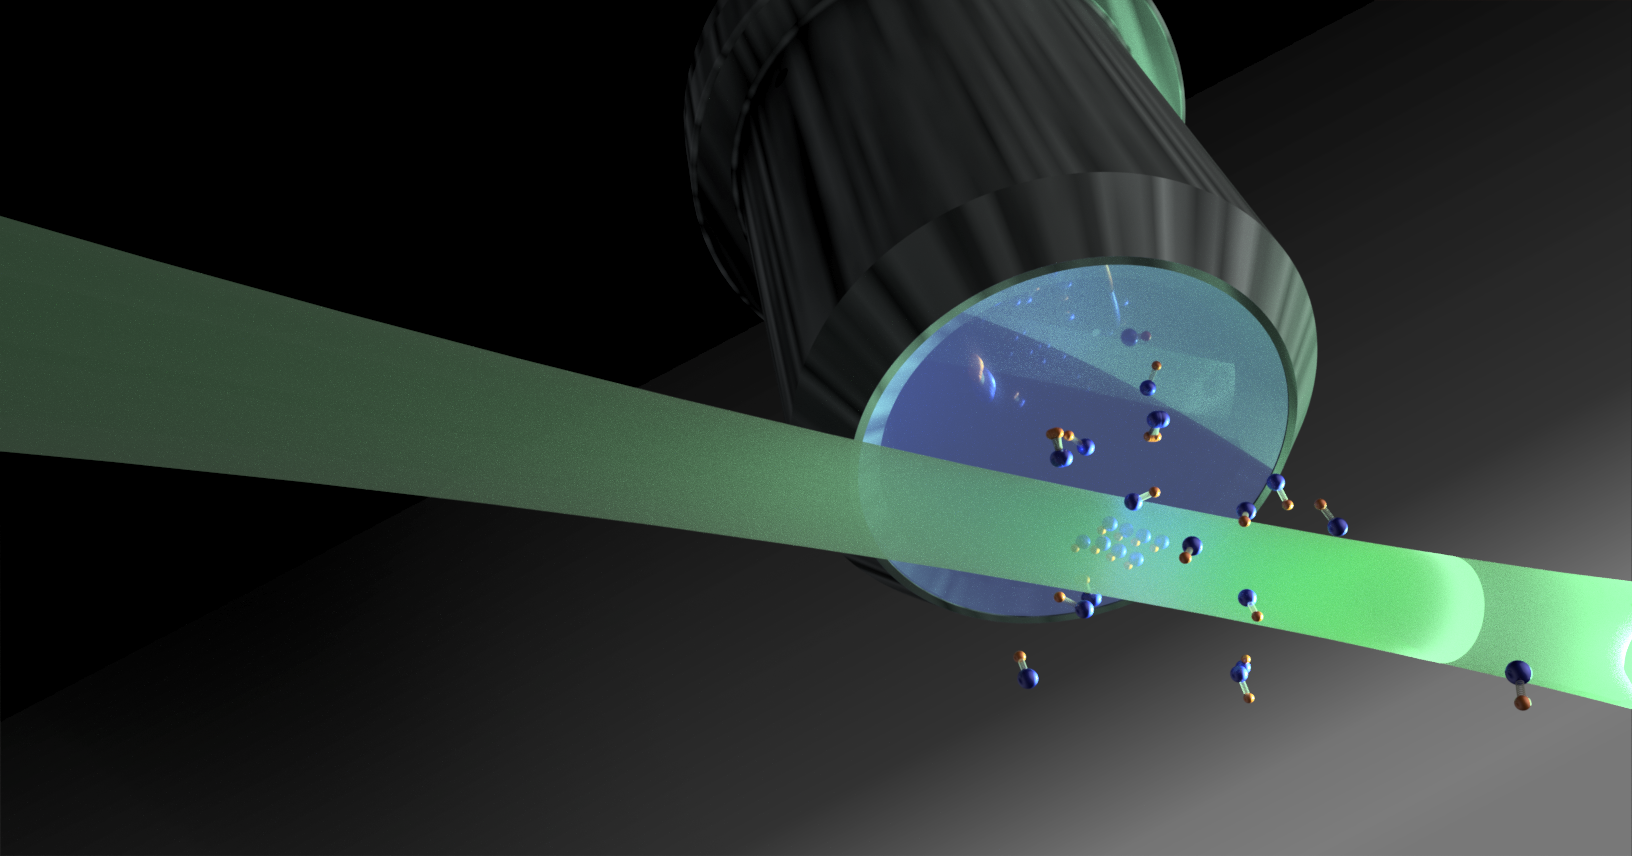
\includegraphics[width=\paperwidth]{front_bg.png}}
  }
  \setbeamercolor{title}{fg=white}
  \setbeamercolor{author}{fg=white}
  \setbeamercolor{institute}{fg=white}
  \setbeamercolor{date}{fg=white}
  \begin{frame}{}
    \titlepage
  \end{frame}
}

%% Motivation
% The long standing goal of our experiment is to create single molecule
% in the optical tweezer.
% By combining the dipole interaction of molecules with the flexibility
% of optical tweezers, we believe this will be a great addition to the
% AMO toolbox for applications like quantum computing
% quantum simulation, quantum chemistry etc.

\begin{frame}{}
  \begin{center}
    \begin{tikzpicture}
      \node[above left, text width=4.5cm] at (0, 0.5) {\begin{block}{Molecules}
          \begin{itemize}
          \item Dipole moment
          \item Rich internal states
          \item $\cdots$
          \end{itemize}
        \end{block}};
      \node[below left, text width=4.5cm] at (0, -0.5) {\begin{block}{Optical tweezers}
          \begin{itemize}
          \item Single site imaging
          \item Single site addressing
          \item Flexible geometry
          \item $\cdots$
          \end{itemize}
        \end{block}};
      \visible<2->{
        \draw[decoration={brace, amplitude=10pt}, decorate, line width=2]
        (0.4, 3) -- (0.4, -4);
        \node[right, align=center] at (0.7, 2) {
          \usebeamercolor[fg]{frametitle}{\small Precision Measurement}\\
          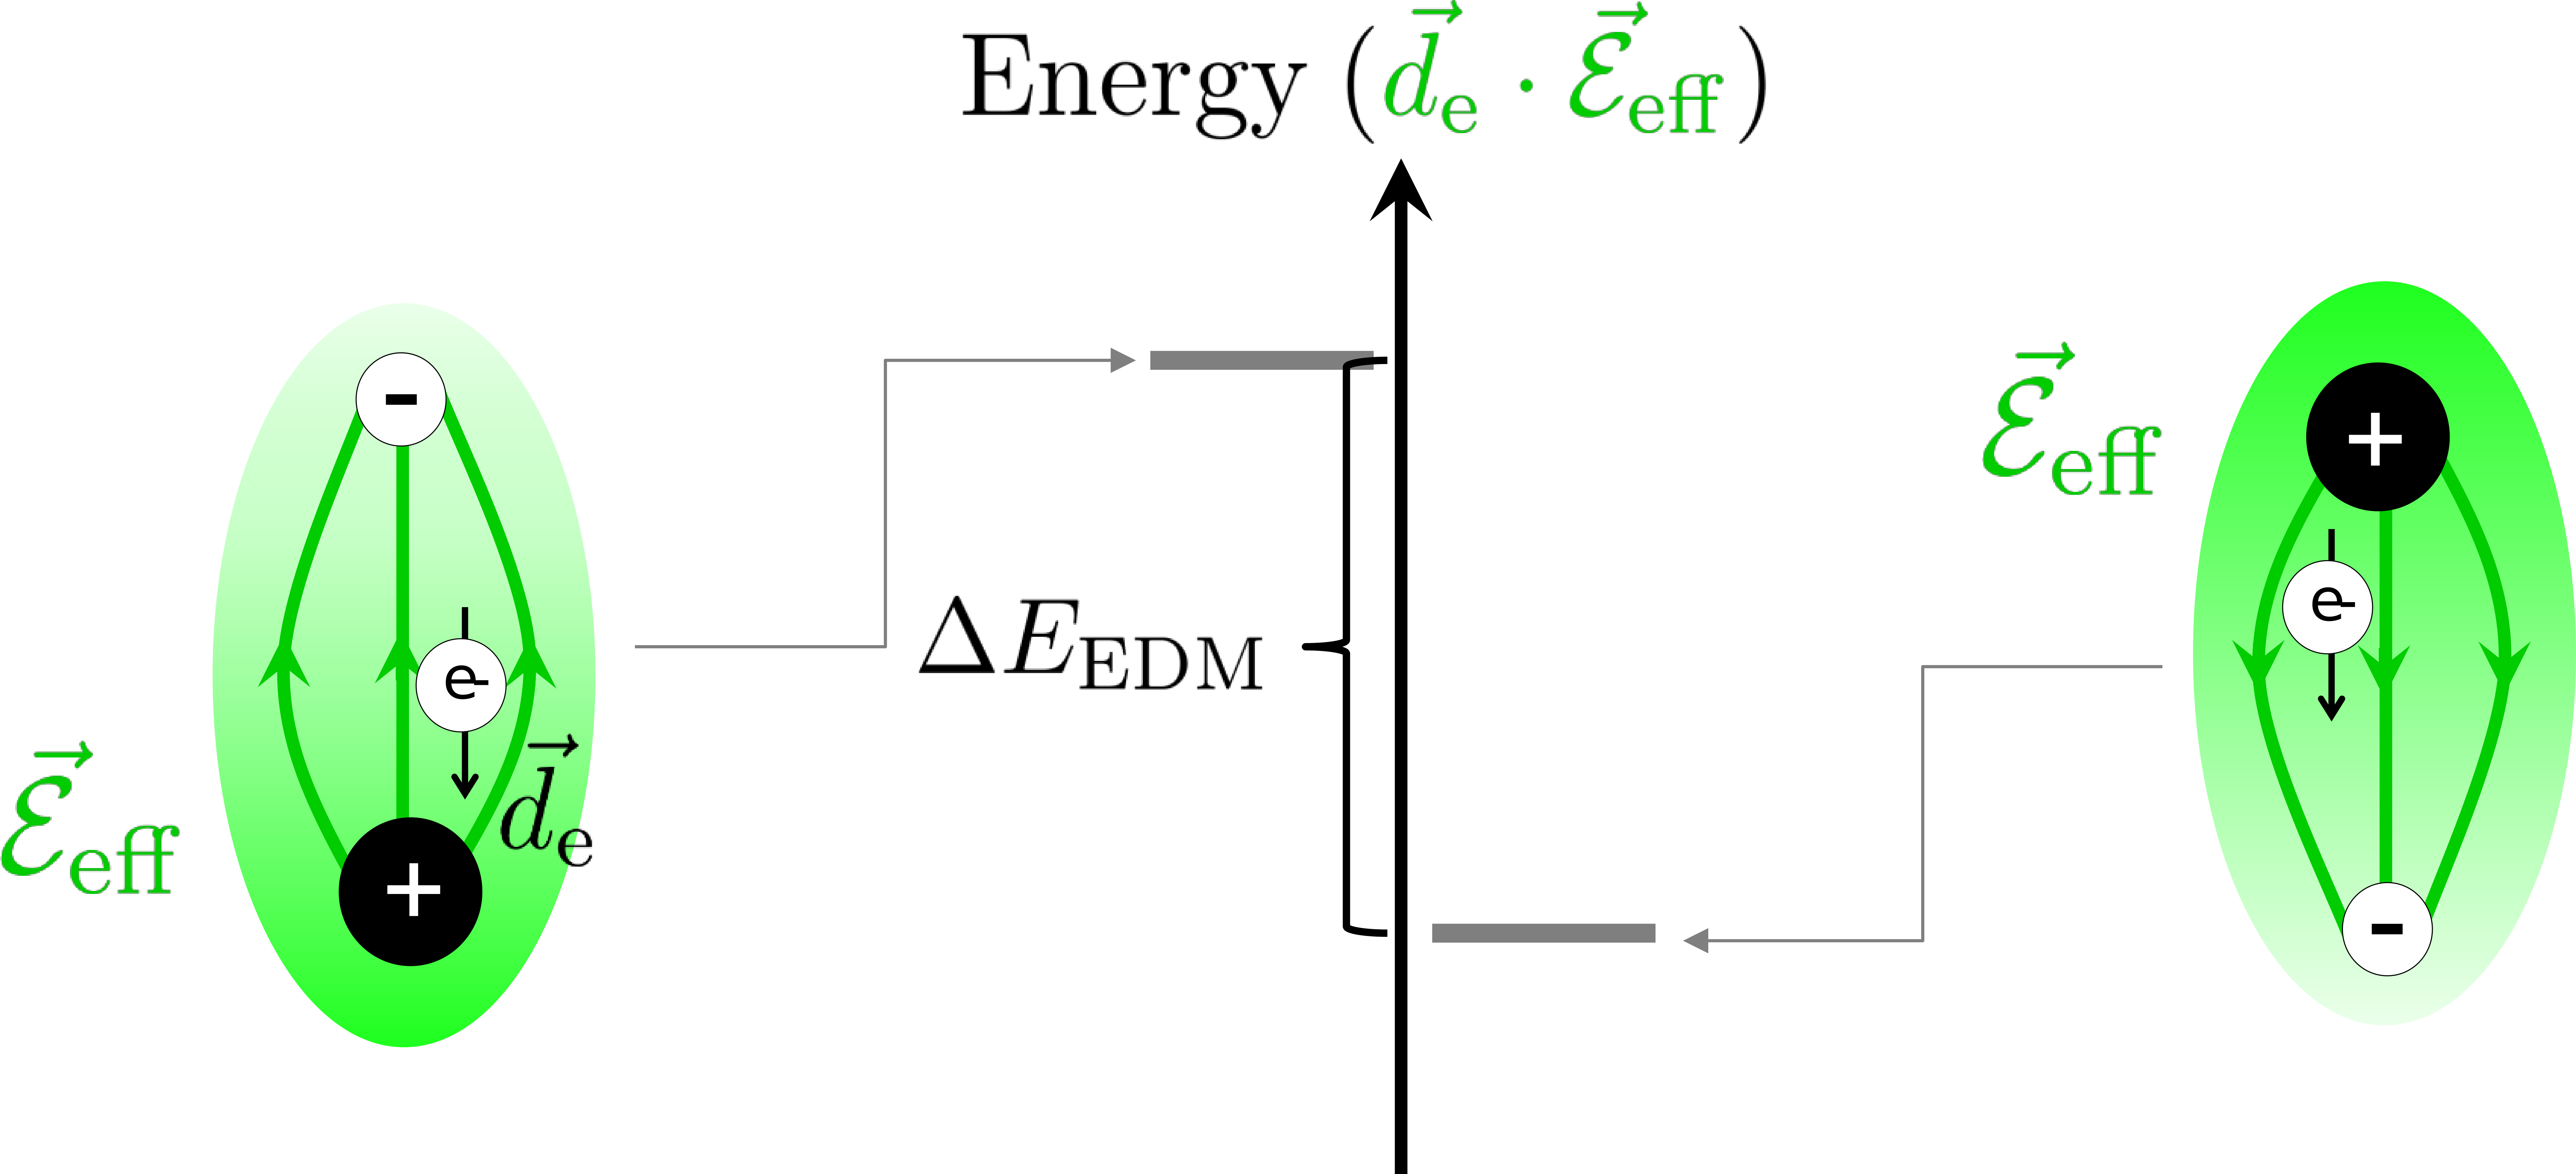
\includegraphics[width=3.6cm]{edm}\\
          {\tiny Science 343, p. 269-272 (2014)}};
        \node[right, align=center] at (4.5, 1.8) {
          \usebeamercolor[fg]{frametitle}{\small Quantum Chemistry}\\
          \includegraphics[width=2.3cm]{quantum_chemistry}\\
          {\tiny Nature 464, 1324 (2010)}};
        \node[right, align=center] at (1.0, -1.7) {
          \usebeamercolor[fg]{frametitle}{\small Quantum Simulation}\\
          \includegraphics[width=2.9cm]{quantum_simulation}\\
          {\tiny Nat. Phys. 2, 341 (2006)}};
        \node[right, align=center] at (4.2, -2.9) {
          \usebeamercolor[fg]{frametitle}{\small Quantum Computing}\\
          \includegraphics[width=2.9cm]{quantum_computing}\\
          {\tiny Phys. Rev. Lett. 97, 33003 (2006)}};
      }
    \end{tikzpicture}
  \end{center}
\end{frame}

%% Molecule from atom
% Our approach for creating and trapping ultracold molecules,
% as you'll hear for many of the other talks in this session,
% is to start from ultracold atoms before coherently transfer them into a molecule.
% This allow us to take advantage of the techniques for cooling and trapping atoms
% without having to implement laser cooling on the molecule.

% In particular, we starts by loading two atoms from MOT in their respective optical tweezers.
% We then use RSC to cool atoms into their 3D motional ground state.
% At this point the atoms are still micros from each other so
% we merge them into the same tweezer adiabatically
% so that we can start turning them into molecules.

\begin{frame}[t]{From atoms to molecules}
  \vspace{-0.5cm}
  \begin{center}
    \begin{tikzpicture}[scale=0.7]
      \visible<1>{
        \shade[ball color=blue!90] (-0.8, -3.7) circle (0.45);
        \shade[ball color=orange!90] (0.3, -3.3) circle (0.3);
        \path (-0.25, -4.3) node[below, align=center] {\textbf{Ultracold atoms}\\\\
          \small{(laser cooling and trapping)}};

        \draw[blue, ->, line width=2] (1.1, -3.5) to [bend left=30]
        node[above=0.2] {\textbf{Coherent transfer}} (8.2, -3.5);

        \shade[ball color=blue!90] (9, -3.6) circle (0.45);
        \shade[ball color=orange!90] (9.4, -3.4) circle (0.3);
        \path (9.2, -4.3) node[below] {\textbf{Ultracold molecule}};
      }
      \visible<2->{
        \only<2->{
          % drawing on different layer does not work with \visibile.
          \mytweezer.drawCsTweezer(0, 0)
          \mytweezer.drawNaTweezer(-1, 0)
          \mytweezer.drawCsAtom(-0.07, 0.08, 0.22)
          \mytweezer.drawNaAtom(-1.06, -0.09, 0.27)

          \mytweezer.drawCsTweezer(0, -3.1)
          \mytweezer.drawNaTweezer(-1, -3.1)
          \mytweezer.drawCsAtom(0.0, -3.1, 0.12)
          \mytweezer.drawNaAtom(-1.0, -3.1, 0.16)

          \mytweezer.drawCsTweezer(-1, -7.0)
          \mytweezer.drawNaAtom(-1.05, -6.87, 0.16)
          \mytweezer.drawCsAtom(-0.95, -7.13, 0.12)
        }

        \fill[white,temporal=<2>{opacity=0.82}{opacity=0}{opacity=0.5}]
        (-1.5, 1.5) rectangle (0.5, -1.5);
        \fill[white,temporal=<3>{opacity=0.82}{opacity=0}{opacity=0.5}]
        (-1.5, 1.5 - 3.1) rectangle (0.5, -1.5 - 3.1);
        \fill[white,temporal=<4>{opacity=0.82}{opacity=0}{opacity=0.5}]
        (-1.5, 1.5 - 7.0) rectangle (-0.5, -1.5 - 7.0);

        \visible<3->{
          \begin{scope}[alt=<3>{opacity=0.7}{opacity=0.35}]
            \draw[orange,dotted,line width=1.2] (-1, -0.4) -- (-1, -2.9);
            \draw[blue,dotted,line width=1.2] (0, -0.15) -- (0, -2.9);
          \end{scope}
        }

        \visible<4->{
          \begin{scope}[alt=<4>{opacity=0.7}{opacity=0.35}]
            \draw[->,orange,line width=1.2] (-1, -3.3) -- (-1, -6.7);
            \draw[->,blue,domain=-3.3:-6.7,smooth,variable=\y,line width=1.2]
            plot ({atan((\y+4.7) * 5) / 170 - 0.5},{\y});
          \end{scope}
        }
        \visible<2>{
          \node[above,align=center] at (7, 0)
          {\usebeamerfont{frametitle}\usebeamercolor[fg]{frametitle}{\Large Loading}};
          \node[below,align=center] at (6.5, -0.5)
          {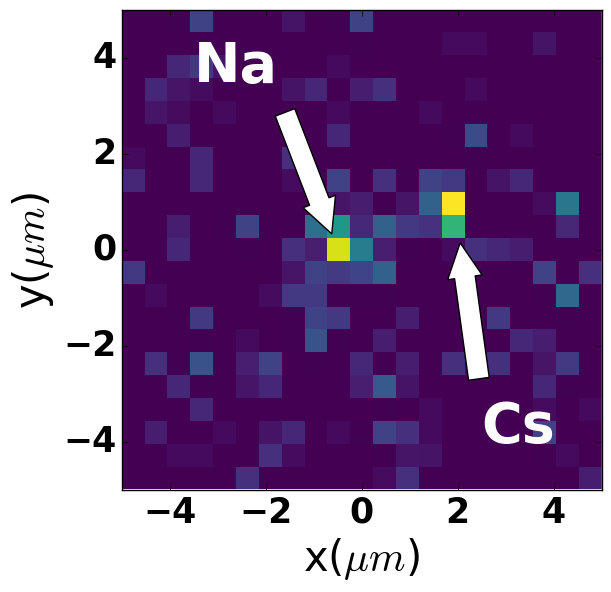
\includegraphics[width=5cm]{../../experiments/nacs_atoms/imgs/single_viridis.png}};
          \node[below,align=center] at (7, -7.5)
          {Loading probability per site: 60\%\\
            Post select on initial and final state.};
        }
        \visible<3>{
          \node[above,align=center] at (7, 0)
          {\usebeamerfont{frametitle}\usebeamercolor[fg]{frametitle}{\Large Cooling}};
          \node[below] at (6.5, -1)
          {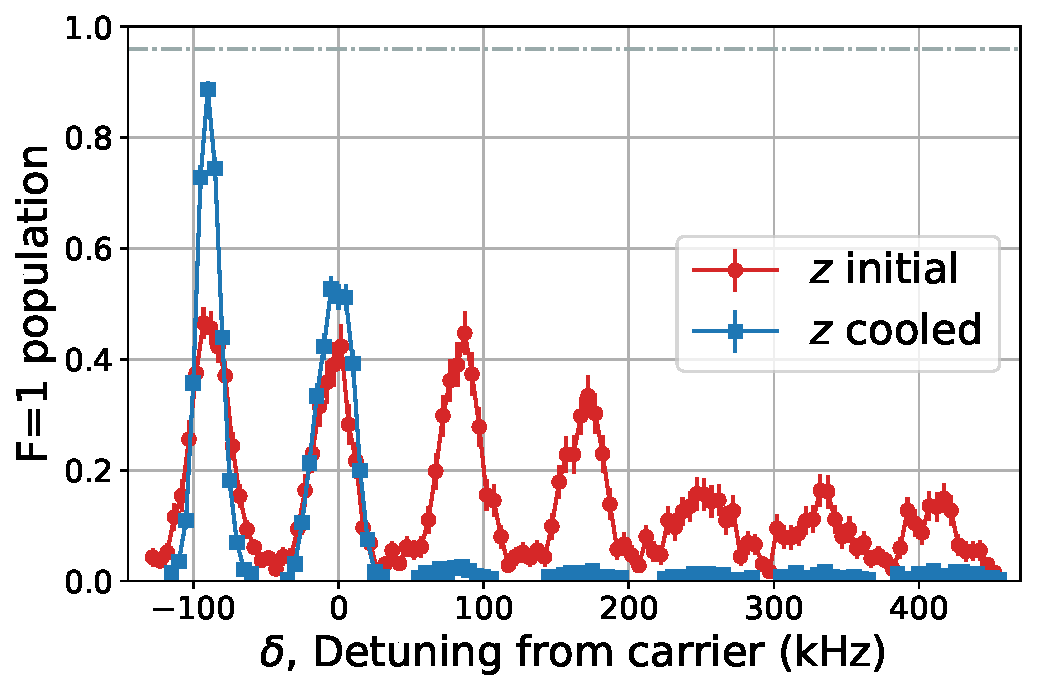
\includegraphics[width=6cm]{spectrum_nolabel_az.pdf}};
          Don't mention axis.
          Explain the sideband spectrum more.
          \only<3>{
            \node[below,align=center] at (7, -7)
            {Cs: 96\% ground state\footnote{Phys. Rev. X 9, 021039}\\
              Na: 94\% ground state\footnote{Phys. Rev. A 97, 063423}};
          }
        }
        \visible<4>{
          \node[above,align=center] at (7, 0)
          {\usebeamerfont{frametitle}\usebeamercolor[fg]{frametitle}{\Large Merging}};
          \draw[orange,line width=1.5] plot[draw,samples=200,domain=4.5:10.5]
          function {-0.22 * exp(-(x - 9)**2 / 0.75**2) + -0.4 * exp(-(x - 6)**2 / 0.75**2) - 1};
          \draw[blue,line width=1.5] plot[draw,samples=200,domain=4.5:10.5]
          function {-1.2 * exp(-(x - 9)**2 / 0.75**2) + 0.45 * exp(-(x - 6)**2 / 0.75**2) - 1};
          \mytweezer.drawNaAtom(6, -1.22, 0.15)
          \mytweezer.drawCsAtom(9, -2.06, 0.11)

          \draw[orange,line width=1.5] plot[draw,samples=200,domain=4.5:10]
          function {-0.22 * exp(-(x - 7.5)**2 / 0.75**2) + -0.4 * exp(-(x - 6)**2 / 0.75**2) - 3.5};
          \draw[blue,line width=1.5] plot[draw,samples=200,domain=4.5:10]
          function {-1.2 * exp(-(x - 7.5)**2 / 0.75**2) + 0.45 * exp(-(x - 6)**2 / 0.75**2) - 3.5};
          \mytweezer.drawNaAtom(6, -3.72, 0.15)
          \mytweezer.drawCsAtom(7.5, -4.56, 0.11)

          \draw[orange,line width=1.5] plot[draw,samples=200,domain=4.5:8.5]
          function {-0.22 * exp(-(x - 6)**2 / 0.75**2) + -0.4 * exp(-(x - 6)**2 / 0.75**2) - 6};
          \draw[blue,line width=1.5] plot[draw,samples=200,domain=4.5:8.5]
          function {-1.2 * exp(-(x - 6)**2 / 0.75**2) + 0.45 * exp(-(x - 6)**2 / 0.75**2) - 6};
          \mytweezer.drawNaAtom(5.9, -6.42, 0.12)
          \mytweezer.drawCsAtom(6.05, -6.6, 0.13)

          \draw[orange,line width=1.5] plot[draw,samples=200,domain=4.5:8.5]
          function {-0.22 * exp(-(x - 6)**2 / 0.75**2) - 8.5};
          \draw[blue,line width=1.5] plot[draw,samples=200,domain=4.5:8.5]
          function {-1.2 * exp(-(x - 6)**2 / 0.75**2) - 8.5};
          \mytweezer.drawNaAtom(6, -8.55, 0.14)
          \mytweezer.drawCsAtom(6, -9.56, 0.11)

          \draw[dotted,line width=2,black!30,opacity=10] (0.3, -3.0) -- (4.5, -0.5);
          \draw[dotted,line width=2,black!30,opacity=10] (-0.7, -7.0) -- (4.5, -9.3);
        }
      }
    \end{tikzpicture}
    \vspace{-2cm}
  \end{center}
\end{frame}

%% Size mismatch
% At this stage, the two atoms are about as closed to each other as they can be
% from the confinement, which is (...). However, in order to make a molecule,
% the two atoms have to be (...) apart and this length scale difference poses the
% biggest challange in our experiment.

\begin{frame}{Wave function size mismatch}
  \begin{center}
    \begin{tikzpicture}
      \shade[ball color=blue!90] (0, 0) circle (0.45);
      \shade[ball color=orange!90] (0.4, 0.2) circle (0.3);
      \draw[<->,line width=1] (-0.45, 0.4) -- (0.35, 0.8);
      \path (-0.05, 0.6) node[rotate=26.565,above=2pt] {$4a_0$};
      \path (0.2, -1.2) node[below] {\textbf{Molecule}};

      \draw[line width=1] plot[samples=200,domain=-2:2,variable=\x] ({\x + 6}, {(\x)^2 * 0.8 - 1.5});
      \draw[line width=2,orange!90!black]
      plot[samples=200,domain=-2:2,variable=\x] ({\x + 6}, {exp(-(\x)^2 * 1.3) - 0.988});
      \draw[line width=0.8] (6 - 0.8, -0.988) -- (6 + 0.8, -0.988);
      \draw[<->,line width=1] (6 - 1, 0.3) -- (6 + 1, 0.3);
      \path (6, 0.3) node[above] {$1000a_0$};
      \path (6, -1.8) node[below] {\textbf{Atom}};
    \end{tikzpicture}
  \end{center}
\end{frame}

% The "tranditional" way of bridging this gap is to use a FB resonance and creating
% a FB molecule first. It works although it relies on finding good FB resonances
% and also typically requires large B field.
% Since it's a tried and work technique, we also have an experiment using this method.
% See [arxiv] and recently accepted by PRL.

% What I am going to talk about today, however, is a different approach that uses only
% optical transitions to go from the atomic state to the molecular state.
% By not relying on FB resonance, this approach is faster, does not require
% a big coil, and most importantly, we hope this can be more generally apply to
% molecules that may not have an accessible/usable FB resonance.
% It's worth pointing out that optical transfer has been previously done.
% However, it was either done incoherently, or it relies on narrow line transition
% in Alkali earth atoms limiting the generality of the approach.

\begin{frame}[t]{Wave function size mismatch}
  \hspace{0.3cm}
  \begin{tikzpicture}[scale=0.8]
    \shade[ball color=blue!90] (0, 0) circle (0.45);
    \shade[ball color=orange!90] (0.4, 0.2) circle (0.3);
    \draw[<->,line width=1] (-0.45, 0.4) -- (0.35, 0.8);
    \path (-0.05, 0.6) node[rotate=26.565,above=2pt] {$4a_0$};
    \path (0.2, -1.2) node[below] {\textbf{Molecule}};

    \draw[line width=1] plot[samples=200,domain=-2:2,variable=\x] ({\x + 4}, {(\x)^2 * 0.8 - 1.5});
    \draw[line width=2,orange!90!black]
    plot[samples=200,domain=-2:2,variable=\x] ({\x + 4}, {exp(-(\x)^2 * 1.3) - 0.988});
    \draw[line width=0.8] (4 - 0.8, -0.988) -- (4 + 0.8, -0.988);
    \draw[<->,line width=1] (4 - 1, 0.3) -- (4 + 1, 0.3);
    \path (4, 0.3) node[above] {$1000a_0$};
    \path (4, -1.8) node[below] {\textbf{Atom}};
  \end{tikzpicture}
  \begin{center}
    \begin{columns}
      \column{5.5cm}
      \begin{center}
        \usebeamercolor[fg]{frametitle}{\textbf{Feshbach molecule}}
      \end{center}
      \begin{itemize}
      \item Requires Feshbach resonance
      \item Usually large magnetic field
      \end{itemize}
      \vspace{0.3cm}
      \visible<2->{
        \begin{center}
          {\usebeamercolor[fg]{frametitle}{Our implementation}}\\
          \small{arXiv:2003.07850}
          \small{(accepted by PRL)}\\
          \small{Poster Q01.00108}
        \end{center}
      }
      \column[t]{6cm}
      \vspace{-6cm}
      \visible<3->{
        \begin{center}
          \usebeamercolor[fg]{frametitle}{\textbf{Optical transfer}}
        \end{center}
        \begin{itemize}
        \item More general
        \item Faster
        \end{itemize}
      }
      \visible<4->{
        \begin{center}
          {\usebeamercolor[fg]{frametitle}{Previous results}}\\
          \begin{itemize}
          \item Rb + Rb\\
            {\small Phys. Rev. Lett. 93, 073002 (2004)}
          \item Sr + Sr\\
            % TODO: reference
          \end{itemize}
        \end{center}
      }
      \visible<5->{
        % The end and restart of center gives a nice spacing here...
        \begin{center}
          {\usebeamercolor[fg]{frametitle}{Limitations}}\\
          \begin{itemize}
          \item Incoherent due to scattering
          \item Using narrow line optical transition
          \end{itemize}
        \end{center}
      }
    \end{columns}
  \end{center}
\end{frame}

%% Raman scheme
% The scheme we use is actually very simple.
% After cooling the atoms into th motional ground state, we shine a pair of
% lasers detuned from an excited state to drive a Raman transition into the
% molecular state and we usually target the least bound molecular state
% which is the most similar to the initial state.

\begin{frame}{Raman transfer}
  \begin{center}
    \begin{tikzpicture}
      \begin{scope}[scale=0.9]
        \draw[->,line width=1.2] (0, 0) -- (0, 8);
        \node[above,rotate=90] at (0, 4) {Energy};
        \draw[->,line width=1.2] (0, 0) -- (7.5, 0);
        \node[below] at (3.75, -0.1) {Internuclear distance};

        \draw[cyan!85!blue] (1.0269 + 0.25, 2.5) -- (7.25, 2.5);

        \draw[line width=1.1,cyan!85!blue]
        plot[samples=200,domain=0.96:7,variable=\x]
        ({\x + 0.25}, {6.8*\x^(-3.4)-6.5*\x^(-1.7) + 2.5});
        \node[cyan!85!blue] at (3.75, 1.0) {$a^3\Sigma^+$};

        \draw[line width=1.1,red]
        plot[samples=200,domain=1:7.5,variable=\x]
        ({\x - 0.75}, {9.2*\x^(-2.5)-9.0*\x^(-1.3) + 7.5});
        \node[above right,red] at (0.55, 7.2) {$c^3\Sigma^+$};

        \draw[red] (1.1576 - 0.75, -1.0595 + 7.5) -- (4.5 - 0.75, -1.0595 + 7.5);
        \draw[black!40,dashed,line width=1] (1 - 0.75, -1.2 + 7.5) -- (5.25 - 0.75, -1.2 + 7.5);

        \mytweezer.drawNaAtom(6.55, 2.6, 0.12)
        \mytweezer.drawCsAtom(7.05, 2.6, 0.10)

        \draw[->,blue!50!orange,line width=0.8] (6.8, 2.7) -- (3.5 - 0.75, -1.2 + 7.5);

        \draw[cyan!85!blue] (1.0793 + 0.25, -0.4631 + 2.5) -- (4.5 + 0.25, -0.4631 + 2.5);
        \mytweezer.drawNaAtom(4.08, 2.15, 0.12)
        \mytweezer.drawCsAtom(4.25, 2.15, 0.10)
        \draw[->,green!80!black,line width=0.8] (3.45 - 0.75, -1.2 + 7.5) -- (4.165, 2.25);
      \end{scope}
    \end{tikzpicture}
  \end{center}
\end{frame}

% Of course nothing is as simple as I show in the real system,
% instead of a 3-state system, we have many more state that can cause
% unwanted effect on the transfer.
% 1. The initial states. We trap our atoms in optical tweezers and there
% % are motional states that are trapping frequency away (~20 kHz).
% % In simple term this means we can't go much faster than 1/omega.
% 2. The final states. Other molecular states. Very far away. Not a problem as long as
% % we obey the speed limit from the initial states.
% 3. The intermediate state. Since we are detuned from the excited state, it doesn't really
% % limit our Rabi frequency. OTOH, these state are electronically excited state and they decay.
% % It's also what we are doing differently from previous approaches.
% % The experiments I've mentioned previously have mainly focused on using an intermediate
% % state that is closed to the dissociation threshold while we picked a deeply bound state
% % as intermediate state for our transfer scheme.
% % Advantage: large coupling to the atomic state. However, there are more
% % and closer other states near the threshold meaning there isn't enough room
% % to detune and reduce the scattering rate. This can be shown in our calculation.

\begin{frame}{Raman transfer}
  \begin{center}
    \begin{tikzpicture}
      \begin{scope}[scale=0.66]
        %% Extra states
        \visible<2-3>{
          \draw (1.0269 + 0.25, 2.5 + 0.1) -- (7.25, 2.5 + 0.1);
          \draw (1.0269 + 0.25, 2.5 + 0.2) -- (7.25, 2.5 + 0.2)
          node[right=0.3] {\small $2\omega=10-50\ \mathrm{kHz}$};
          \draw (1.0269 + 0.25, 2.5 + 0.3) -- node[above] {$\vdots$} (7.25, 2.5 + 0.3);
        }

        \visible<4>{
          \draw (1.2 + 0.25, -1 + 2.5) -- (2.65 + 0.25, -1 + 2.5);
          \node[below] at (1.6 + 0.25, -0.7 + 2.5) {$\vdots$};
        }

        \visible<5->{
          \draw (1.1102 - 0.75, -0.7720 + 7.5) -- node[above] {$\vdots$}
          (6 - 0.75, -0.7720 + 7.5);
          \draw (1.2 - 0.75, -1.4 + 7.5) -- (3.4 - 0.75, -1.4 + 7.5);
          \node[below] at (1.85 - 0.75, -1.1 + 7.5) {$\vdots$};
        }
        \visible<6->{
          \draw[snakearrow] (5 - 0.75, -0.7720 + 7.5) -- (6.5 - 0.75, -2 + 7.5);
          \draw[snakearrow] (2.5 - 0.75, -1.4 + 7.5) -- (2.8 - 0.75, -3 + 7.5);
        }

        %% 3-states Raman
        \draw[->,line width=1.2] (0, 0) -- (0, 8);
        \node[above,rotate=90] at (0, 4) {Energy};
        \draw[->,line width=1.2] (0, 0) -- (7.5, 0);
        \node[below] at (3.75, -0.1) {Internuclear distance};

        \draw[cyan!85!blue] (1.0269 + 0.25, 2.5) -- (7.25, 2.5);
        \draw[cyan!85!blue] (1.0793 + 0.25, -0.4631 + 2.5) -- (4.5 + 0.25, -0.4631 + 2.5);

        \draw[line width=1.1,cyan!85!blue]
        plot[samples=200,domain=0.96:7,variable=\x]
        ({\x + 0.25}, {6.8*\x^(-3.4)-6.5*\x^(-1.7) + 2.5});
        \node[cyan!85!blue] at (3.75, 1.0) {$a^3\Sigma^+$};

        \draw[line width=1.1,red]
        plot[samples=200,domain=1:7.5,variable=\x]
        ({\x - 0.75}, {9.2*\x^(-2.5)-9.0*\x^(-1.3) + 7.5});
        \node[above right,red] at (0.55, 7.2) {$c^3\Sigma^+$};

        \draw[red] (1.1576 - 0.75, -1.0595 + 7.5) -- (4.5 - 0.75, -1.0595 + 7.5);

        \mytweezer.drawNaAtom(6.55, 2.6, 0.12)
        \mytweezer.drawCsAtom(7.05, 2.6, 0.10)
        \mytweezer.drawNaAtom(4.08, 2.15, 0.12)
        \mytweezer.drawCsAtom(4.25, 2.15, 0.10)

        \draw[black!40,dashed,line width=1] (1 - 0.75, -1.2 + 7.5) -- (5.25 - 0.75, -1.2 + 7.5);
        \draw[->,blue!50!orange,line width=0.8] (6.8, 2.7) -- node[right] {$\Omega_{up}$}
        (3.5 - 0.75, -1.2 + 7.5);
        \draw[->,green!80!black,line width=0.8] (3.45 - 0.75, -1.2 + 7.5) --
        node[left] {$\Omega_{down}$} (4.165, 2.25);
      \end{scope}
      \visible<2->{
        \node[below right, text width=6.5cm, align=left] at (5, 6) {\begin{itemize}
          \item<3-> No faster than $20-100\ \mu s$
          \item<6-> Additional scattering.
          \end{itemize}
          % Extra {} around \visible that is aparently needed to make \node happy.
          {\visible<7->{
              \begin{center}
                \usebeamercolor[fg]{frametitle}{\textbf{Near threshold states}}
              \end{center}
              \begin{itemize}
              \item Closely spaced
              \item Stronger coupling ($\Omega_{up}$)
              \item Easier to find
              \end{itemize}
            }}
          {\visible<8->{
              \begin{center}
                \usebeamercolor[fg]{frametitle}{\textbf{Deeply states}}
              \end{center}
              \begin{itemize}
              \item Sparsely spaced
              \item Allow larger detuning
              \item Lower scattering
              \end{itemize}
            }}
        };
      }
    \end{tikzpicture}
  \end{center}
\end{frame}

% % Here you see the Raman Rabi frequency and the scattering rate calculated for
% % Raman beam detuned from two different states.
% % .....
% % Showing that even though at the same deuning the Raman Rabi frequecy is lower for the
% % deeply bound state, we can detune more and win on the Raman Rabi frequency/scattering rate
% % ratio.

\begin{frame}[t]{Raman transfer}
  % TODO: near threshold vs deeply bound plot
  \begin{center}
    \begin{columns}
      \column{5.5cm}
      \begin{center}
        \usebeamercolor[fg]{frametitle}{\textbf{Near threshold states}}
      \end{center}
      \column{5.5cm}
      \begin{center}
        \usebeamercolor[fg]{frametitle}{\textbf{Deeply bound states}}
      \end{center}
    \end{columns}
  \end{center}
\end{frame}

%% State selection
% So that's theory is all good, what about the experiment.
% To be more particular. We use 33+22 initial state.
% We found the bound state thanks to Jeremy's prediction based on our
% interaction shift [ref] and FB rersonance [ref] measurement.
% The excited state we use is the v=0 bound state for the c3sigma potential.

% Thanks to the prediction, it didn't take too long for us to find the resonance.
% (Show Raman spectrum). It's ~1MHz from where the prediction was, which is pretty good.
% More importantly though, this is taken with a (...) pulse time and we got a FWHM of
% (...) which is what you'll expect from a Fourier limited linewidth.
% This suggest that we are at least very closed to the coherent regime where the
% Raman Rabi frequency exceeds the scattering rate.
% Next we switched to scanning the time on resonance.
% See oscillation!!

\begin{frame}[t]{Experiment}
  \begin{center}
    \vspace{-1cm}
    \begin{tikzpicture}
      \begin{scope}[scale=0.6]
        \draw[->,line width=1.2] (0, 0) -- (0, 8);
        \node[above,rotate=90] at (0, 4) {Energy};
        \draw[->,line width=1.2] (0, 0) -- (7.5, 0);
        \node[below] at (3.75, -0.5) {Internuclear distance};

        \draw[cyan!85!blue] (1.0269 + 0.25, 2.5) -- (7.25, 2.5)
        node[above, align=left] {{\visible<2->{\scriptsize $F_{Cs}=3,m_F=3$}}\\
          {\visible<2->{\scriptsize $F_{Na}=2,m_F=2$}}};
        \draw[cyan!85!blue] (1.0793 + 0.25, -0.4631 + 2.5) -- (4.5 + 0.25, -0.4631 + 2.5)
        node[below right] {{\visible<3->{\scriptsize $E\approx-770\ MHz$ \footnote{Phys. Rev. Research 2, 023108 (2020)}}}};

        \draw[line width=1.1,cyan!85!blue]
        plot[samples=200,domain=1:7,variable=\x]
        ({\x + 0.25}, {6.8*\x^(-3.4)-6.5*\x^(-1.7) + 2.5});
        \node[cyan!85!blue] at (3.75, 1.0) {$a^3\Sigma^+$};

        \draw[line width=1.1,red]
        plot[samples=200,domain=1:7.5,variable=\x]
        ({\x - 0.75}, {9.2*\x^(-2.5)-9.0*\x^(-1.3) + 7.5});
        \node[above right,red] at (0.55, 7.2) {$c^3\Sigma^+$};

        \draw[red] (1.4 - 0.75, 5.6) -- (2.35 - 0.75, 5.6)
        node[right=0.2] {{\visible<4->{\small $v=0$}}};

        \draw[black!40,dashed,line width=1] (0.25, 5.25) -- (7.25, 5.25);

        \begin{scope}[shift={(-1.8, 0)}]
          \mytweezer.drawNaAtom(6.55, 2.6, 0.12)
          \mytweezer.drawCsAtom(7.05, 2.6, 0.10)

          \mytweezer.drawNaAtom(4.08, 2.15, 0.12)
          \mytweezer.drawCsAtom(4.25, 2.15, 0.10)

          \draw[->,green!80!black,line width=2] (6.8, 2.7) -- (5.5, 5.25);
          \draw[->,green!80!black,line width=2] (5.45, 5.25) -- (4.165, 2.25)
          node[midway, left, align=left] {{\visible<5->{\small $\approx1038\mathrm{nm}$}}\\
            \ {\visible<5->{\small Tweezer}}};
        \end{scope}
      \end{scope}
      \visible<6> {
        \node[right] at (5.2, 4.2) {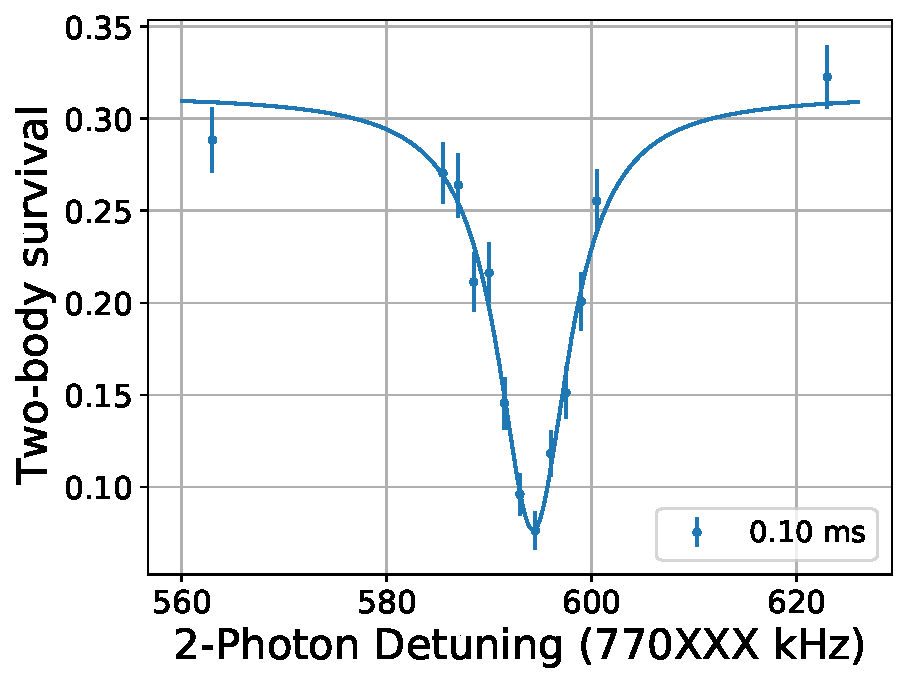
\includegraphics[width=5.5cm]{../../experiments/nacs_202003/imgs/fit_20200326_005204_raman_3322_2_damop_f.pdf}};
      }
      \visible<7-> {
        \node[right] at (5.2, 4.2) {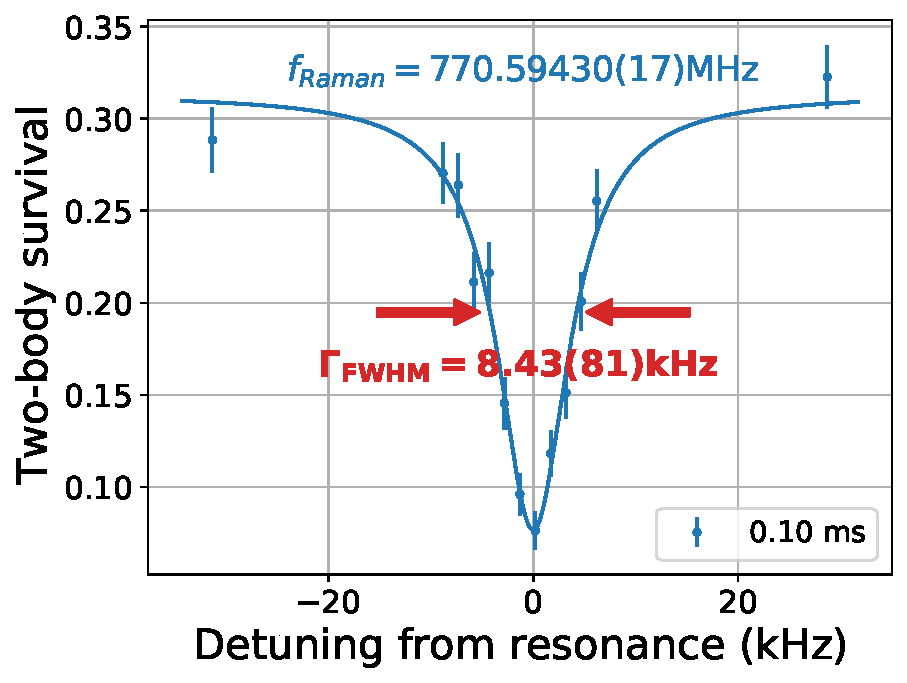
\includegraphics[width=5.5cm]{../../experiments/nacs_202003/imgs/fit_20200326_005204_raman_3322_2_damop_f_text.pdf}};
      }
      \visible<8-> {
        \node[right] at (5.2, -0.5) {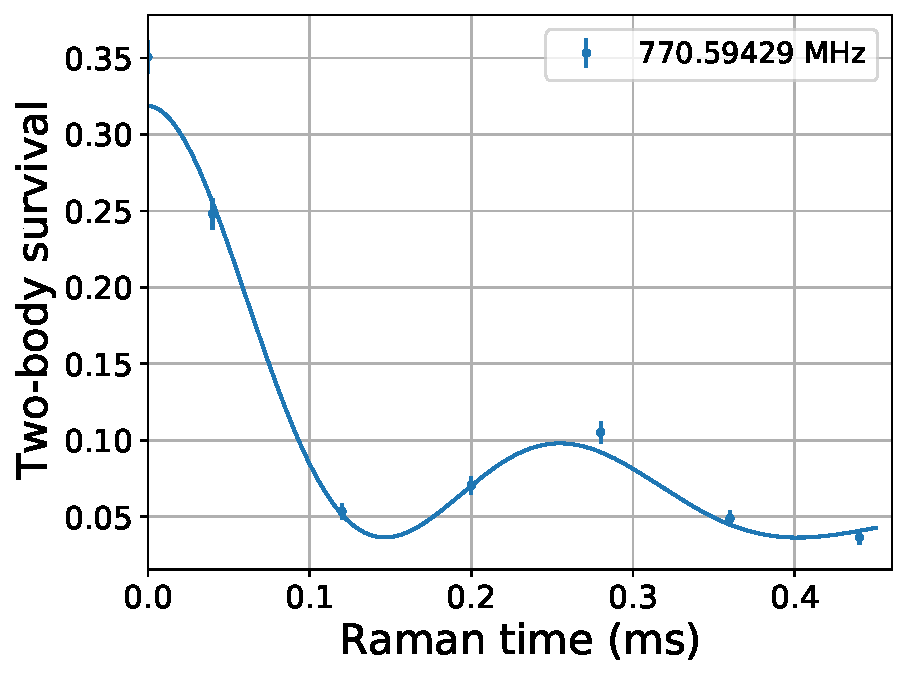
\includegraphics[width=5.5cm]{../../experiments/nacs_202003/imgs/fit_20200326_005204_raman_3322_2_damop_t.pdf}};
      }
    \end{tikzpicture}
    \vspace{-1cm}
  \end{center}
\end{frame}

%% Next
% We are currently working on, with obvious difficulty, improving our signal,
% by improving the fidelity of our sequence and by tweaking transfer parameters.
% It's also worth noting that the contrast isn' great, to put it mildly, much
% worse than the prediction from the Raman Rabi frequency/scattering ratio from calculation.
% Fortunately, as I mentioned earlier, our parallel effort for making FB molecule
% also succeeded recently and is showing a decent lifetime of 4-5 ms,
% so we'll be able to work on transfering to molecular ground state from FB molecule
% as we are investigating the lifetime issue.

\begin{frame}[t]{Outlook}
  \begin{center}
    \vspace{-0.7cm}
    \begin{tikzpicture}
      \node[left, text width=5.5cm, align=left] at (0, 2) {\begin{itemize}
        \item<1-> Molecule lifetime.
        \item<2-> Improve signal contrast.
        \item<3-> Feshbach molecule.\\
          \vspace{0.3cm}
          \small{arXiv:2003.07850}\\
          \small{Poster Q01.00108}
        \end{itemize}
      };
      \node[right] at (0.1, 2) {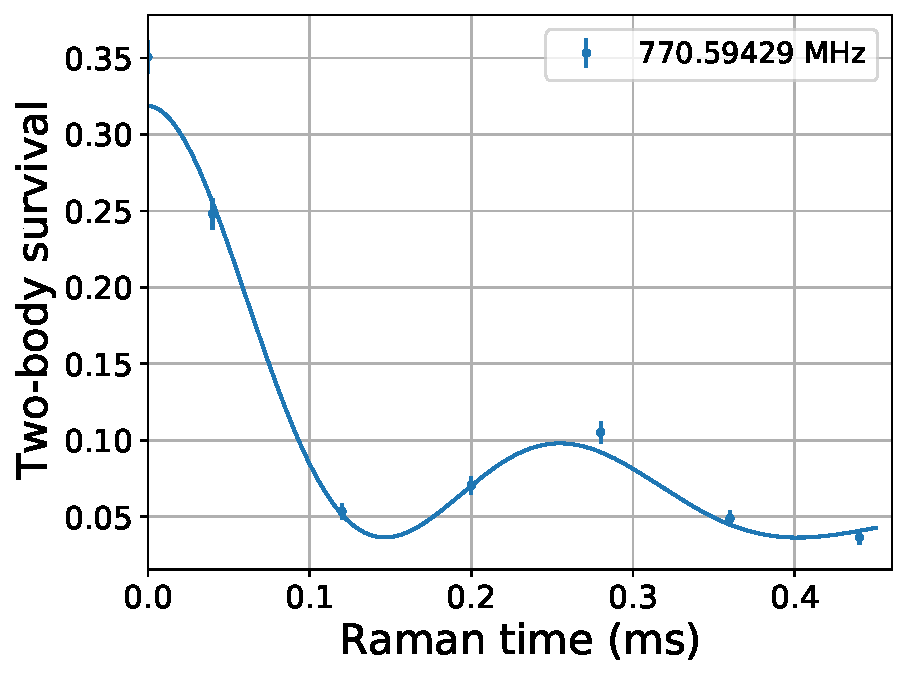
\includegraphics[width=5.5cm]{../../experiments/nacs_202003/imgs/fit_20200326_005204_raman_3322_2_damop_t.pdf}};
      \visible<2-> {
        \node[left] at (-0.1, -2) {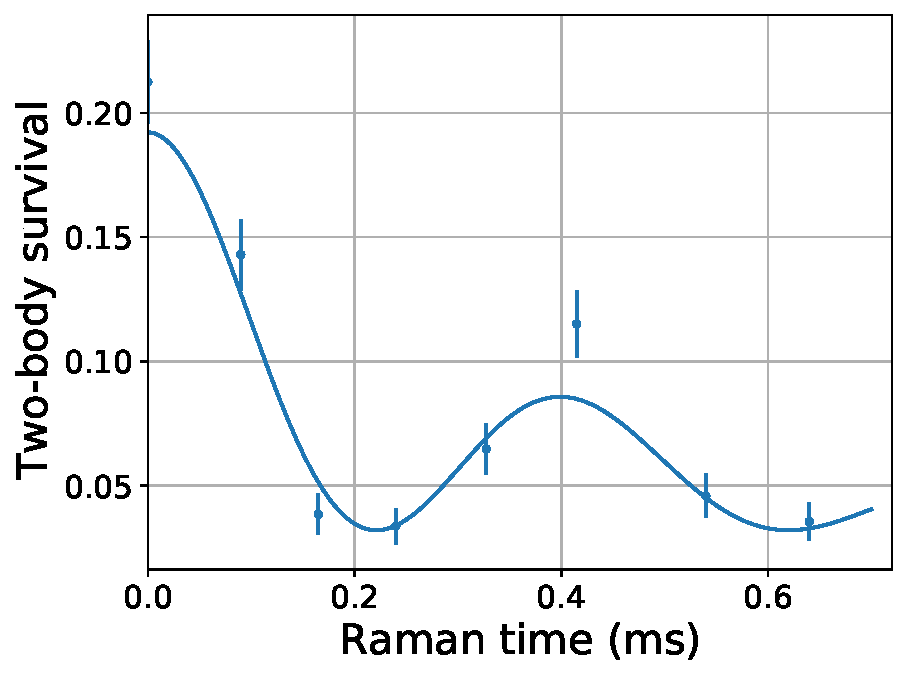
\includegraphics[width=5.5cm]{../../experiments/nacs_202005/imgs/fit_20200524_161707_raman_3322_damop_t.pdf}};
      }
      \visible<3-> {
        \node[right] at (0.1, -2) {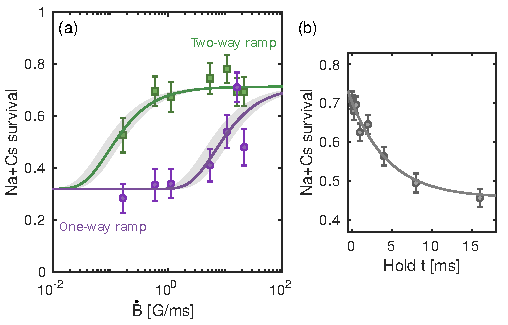
\includegraphics[width=5.5cm]{fb_molecules.pdf}};
      }
    \end{tikzpicture}
  \end{center}
\end{frame}

\begin{frame}{}
\end{frame}

\end{document}
